\subsection{Funções Limitadas}

\begin{definition}
	Seja $f: D \subset \R \to \R$ uma função.
\begin{enumerate}[(i)]
  \item $f$ é \emph{limitada superiormente} se existe $M \in \R$ tal
  que $f(x) \leq M$ para todo $x \in D$;
  \item $f$ é \emph{limitada inferiormente} se existe $M \in \R$ tal
  que $f(x) \geq M$ para todo $x \in D$;
  \item $x_0 \in D$ é um \emph{ponto de máximo absoluto} de $f$ se
  $f(x_0) \geq f(x)$ para todo $x \in D$;
  \item $x_0 \in D$ é um \emph{ponto de mínimo absoluto} de $f$ se
  $f(x_0) \leq f(x)$ para todo $x \in D$;
  \item $x_0 \in D$ é um \emph{ponto de máximo local} de $f$ se
  existe $r>0$ tal que $f(x_0) \geq f(x)$ para todo $x \in D \inter \paren{x_0 - r , x_0+r}$;
  \item $x_0 \in D$ é um \emph{ponto de mínimo local} de $f$ se
  existe $r>0$ tal que $f(x_0) \leq f(x)$ para todo $x \in D \inter \paren{x_0 - r ,
  x_0+r}$;
  \item $x_0 \in D$ é um \emph{extremo absoluto} (respctivamente, \emph{local}) de $f$ se $x_0$ é um ponto de máximo ou mínimo absoluto (respctivamente, local) de $f$.
\end{enumerate}
\end{definition}

\begin{remark}
	No contexto da definição anterior, quando $x_0$ é um ponto de máximo (ou mínimo) de $f$, é comum dizermos que o ponto $\paren {x_0 , f(x_0)}$ é um ponto de máximo (ou mínimo), fazendo referência ao ponto do gráfico de $f$. Ademais, podemos dizer que há um máximo (ou mínimo) em $x_0$ e que $f(x_0)$ é o valor máximo (ou mínimo) da função $f$. Tais termos podem se referir a extremos absolutos ou locais.
\end{remark}

\begin{example}
	A função $h : \left( -1 ; 6 \right] \to \R$, cujo gráfico é esboçado
na Imagem~\ref{img:funcao-limitada-descontinua}, é definida por:
%
$$h(x) = \begin{cases}
								3x-x^2 & \ \text{ se } \ x\leq 2 \\
								\modu{x-4} +1 & \ \text{ se } \ 2 < x \leq 5 \\
								2 & \ \text{ se } \ x > 5 \\
								\end{cases}.$$
%
\begin{figure}[H]
	\centering
	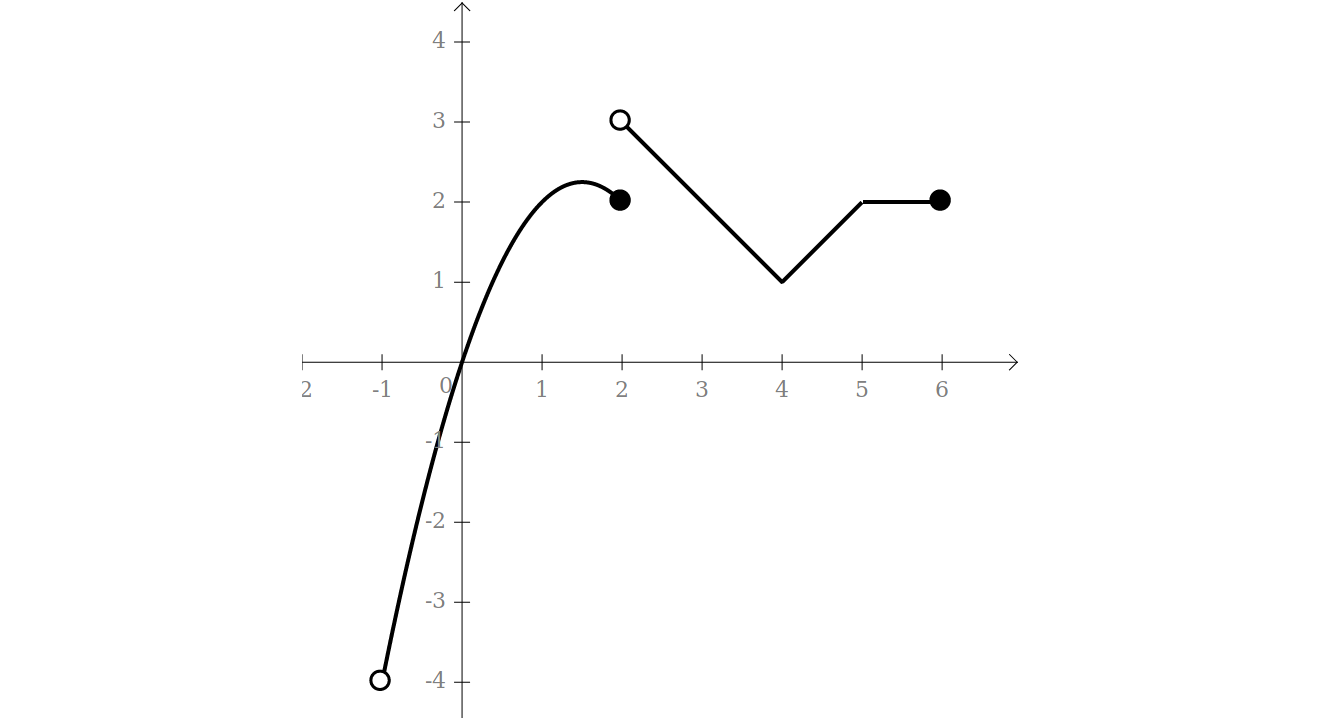
\includegraphics[scale=0.3]{\imgdirfromsection/funcao-limitada-descontinua.png}
	\caption{Gráfico da função $h$.}
	\label{img:funcao-limitada-descontinua}
\end{figure}
%
Identifique, pelo gráfico, os intervalos de monotonicidade e os extremos locais e absolutos de $h$.
\end{example}

\begin{solution}
	A partir do gráfico, pode-se perceber que a função $h$ é crescente nos intervalos $(-1;1{,}5]$ e $[4;5]$,
	decrescente em $[1,5; 2]$ e $(2;4]$ e constante em $[5;6]$.     
	Também por observação do gráfico da função, conclui-se que o ponto $(1{,}5; 2{,}25)$ é um máximo local,
	e o ponto $(4,1)$ é um mínimo local. 
	Além disso, todos os pontos tais que $x \in [5;6]$ são máximos locais,
	e todos os pontos tais que $x \in (5; 6]$ são mínimos locais.
	A função não possui extremos absolutos.

	Na solução dada, alguns fatos podem causar certa confusão. 
	Assim, serão feitas, a seguir, algumas observações baseadas na análise do gráfico para elucidá-los.
	%
	\begin{enumerate}[(a)]
		\item $-1$ não está presente no intervalo de crescimento $(-1;1{,}5]$ por não pertencer ao domínio da função;
		\item \label{item:intervalo-crescimento} $1{,}5$ deve estar no intervalo de crescimento $(-1;1{,}5]$. 
		Note que, para quaisquer $x_1, x_2 \in (-1;1{,}5]$, é verdade que $x_1 < x_2$ implica $h(x_1) < h(x_2)$,
		uma vez que a função é crescente nesse intervalo. 
		Em particular, como $1{,}5$ é o maior dos valores de $(-1;1{,}5]$, 
		temos que $x_1 < 1{,}5$ implica $h(x_1) < h(1{,}5)$;
		\item Analogamente ao item \ref{item:intervalo-crescimento},
		é necessário que $1{,}5$ e $2$ estejam no intervalo de decrescimento $[1,5; 2]$.
		A análise é similar para os extremos dos outros intervalos fechados;
		\item $2$ não deve fazer parte do intervalo de decrescimento $(2; 4]$, 
		pois há uma bola aberta nesse intervalo. 
		Se $2$ pertencesse ao intervalo, teríamos, devido à definição de função decrescente,
		que $2<2{,}1$ implicaria em $2 = h(2) > h(2{,}1) = 2{,}9$. 
		Essa implicação claramente é falsa;
		\item \label{item:minimo-local} O fato de que há um mínimo local quando $x = 4$ se dá pois $4$ é o maior valor de um intervalo de decrescimento e o menor de um intervalo de crescimento. 
		Em outras palavras, em $x=4$, a função que estava decrescendo em $(2;4]$ passa a crescer em $[4;5]$,
		atingindo o menor valor localmente nessa mudança de comportamento da monotonicidade. 
		É comum que mudanças da monotonicidade da função determinem extremos locais.
		No item \ref{item:minimo-local-formal}, é demonstrado que, de fato, há um mínimo local em $x=4$.
		\item A justificativa para a existência de um máximo local em $x=1{,}5$ é análoga à do item \ref{item:minimo-local};
		\item Em todo o intervalo $[5; 6]$, em que a função é constante, 
		os pontos são máximos locais e mínimos locais, exceto pelo fato de que não há mínimo local em $x=5$. 
		Para qualquer $x_0\in (5;6]$, existe um intervalo $(x_0 - r; x_0+r)$ em torno de $x_0$ tal que $f(x)= f(x_0)$ para todo $x \in (x_0 - r; x_0+r) \inter D$, em que $D = \left(-1,6\right]$.
		Note que $f(x)= f(x_0)$ implica tanto $f(x) \leq f(x_0)$ quanto $f(x_0)\leq f(x)$, 
		o que justifica a existência dos mínimos e máximos locais em $(5;6]$. 
		Quando $x_0=5$, conseguimos concluir que $f(x) \le f(x_0)$ mas não $f(x_0) \le f(x)$, 
		pois em qualquer intervalo $(5 - r; 5+r)$ existe $x < 5$ tal que $f(x) < f(5)$.
		Assim, em $x_0=5$ há máximo local mas não mínimo local;
		\item \label{item:minimo-local-formal} Tendo, como verdade, que a função é decrescente em $(2; 4]$ e crescente em $[4; 5]$, 
		provemos que ocorre um mínimo local em $x=4$. Para tanto, precisamos mostrar que existe $r>0$ tal que, 
		para todo $x \in (4-r; 4+r)$, vale $h(4) \leq h(x)$. 
		Tome $r=1$, e seja $x \in (4-1; 4+1) = (3; 5)$. 
		Separaremos, em três casos possíveis para $x$, a verificação de que $h(4) \leq h(x)$. 
		Caso $x \in (3; 4)$, note que $x, 4 \in (2; 4]$, um intervalo de decrescimento da função. 
		Assim, como $x<4$, então $h(4)< h(x)$, o que implica que $h(4) \leq h(x)$. 
		Agora, caso $x \in (4; 5)$, note que $x, 4 \in [4; 5]$, um intervalo de crescimento da função. 
		Assim, como $4<x$, então $h(4)< h(x)$, e, consequentemente, $h(4)\le h(x)$.
		Finalmente, caso $x=4$, é óbvio que $h(4)=h(x)$, o que também implica que $h(4)\le h(x)$. 
		Portanto, em $x=4$ há um mínimo local para a função $h$.
	\end{enumerate}
\end{solution}

\begin{onlineact}
	\khan{https://pt.khanacademy.org/math/algebra/algebra-functions/positive-negative-increasing-decreasing-intervals/e/increasing-decreasing-intervals-of-functions}{Intervalos Crescentes e Decrescentes}.
\end{onlineact}

\begin{onlineact}
	\khan{https://pt.khanacademy.org/math/algebra/algebra-functions/maximum-and-minimum-points/e/recognize-maxima-and-minima}{Mínimos e Máximos Relativos}.
\end{onlineact}

\begin{onlineact}
	\khan{https://pt.khanacademy.org/math/algebra/algebra-functions/maximum-and-minimum-points/e/recognize-absolute-maxima-and-minima}{Mínimos e Máximos Absolutos}.
\end{onlineact}